\documentclass{beamer}
\usepackage{bm,mathtools,multirow}%,transparent}

\definecolor{myblue}{rgb}{0.05,0.32,0.63}
\everymath{\color{myblue}}
\renewcommand{\arraystretch}{1.2}

\title{\vskip5mm Application of smoothed particle hydrodynamics to a ballistic gelatine sample high-speed impact}
\author{\vskip-5mm Lud\v{e}k Hyn\v{c}\'{\i}k}
\institute{New Technologies - Research Centre \\ University of West Bohemia \\ Czech Republic}
\date{\scriptsize Computational Biomechanics for Medicine XVIII \\ Virtual workshop (Perth, Australia) \\ 1 October 2023}

\usepackage{tikz}
%\titlegraphic{ 
\logo{ 
\begin{tikzpicture}[overlay,remember picture];
\node[left=0.5cm] at (current page.32){\includegraphics[width=3cm]{Figures/logo_NTC}};
\end{tikzpicture}
}

\begin{document}

%%%%%%%%%%%%%%%%%%%%%%%%%%%%%%%%%%%%%%%%%%%%%%%%%%%%%%
\begin{frame}
\titlepage
\begin{tikzpicture}[overlay,remember picture];
\node[left=9cm] at (current page.32){
\includegraphics[width=3cm]{Figures/logo_miccai_2023}};
\end{tikzpicture}
\end{frame}

%%%%%%%%%%%%%%%%%%%%%%%%%%%%%%%%%%%%%%%%%%%%%%%%%%%%%%
\begin{frame}
\frametitle{Content}
\begin{columns}[onlytextwidth,T]
\begin{column}{0.55\textwidth}
\tableofcontents[sections=1-3]
\end{column}
\begin{column}{0.45\textwidth}
\tableofcontents[sections=4-6]
\end{column}
\end{columns}
\end{frame}	

%%%%%%%%%%%%%%%%%%%%%%%%%%%%%%%%%%%%%%%%%%%%%%%%%%%%%%
\section{Introduction}

%%%%%%%%%%%%%%%%%%%%%%%%%%%%%%%%%%%%%%%%%%%%%%%%%%%%%%
\subsection{Motivation}

\begin{frame}
\frametitle{Introduction}
\begin{itemize}
\item Institute of Criminalistics (ICP), Prague (Czech Republic)
\item Penetrating ballistic impact \\ for estimating consequences \\ and severity of gunshot wounds
\item Ethics motivates for using \\ substituting matter \\ and numerical modelling
\item Ballistic gelatine correlated well \\ to human muscle tissue
\item Smoothed particle hydrodynamics
\begin{itemize}
\item Ballistic gelatine highly sensitive to strain rate and temperature
\item Behaving as shear thickening fluid at high shear rates
\item Large deformations and material discontinuities
\end{itemize}
\item Numerical model of ballistic gelatine for virtual testing
\end{itemize}
\begin{tikzpicture}[overlay,remember picture];
\node[left=5mm] at (current page.5){\begin{minipage}[c]{5cm}\centering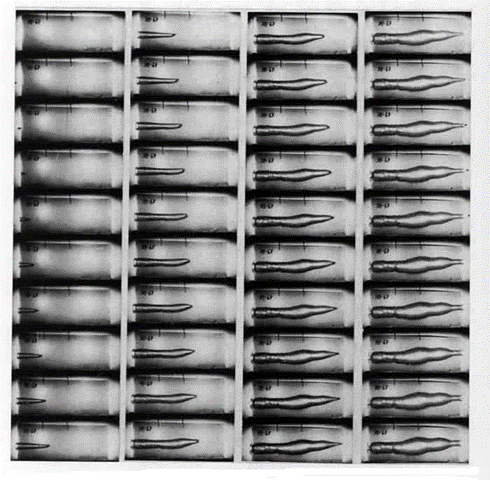
\includegraphics[width=42mm]{Figures/presentation_canal} \\ \vspace{-2mm}{\scriptsize\it Source : ICP}\end{minipage}};
\end{tikzpicture}
\end{frame}

%%%%%%%%%%%%%%%%%%%%%%%%%%%%%%%%%%%%%%%%%%%%%%%%%%%%%%
\section{Smoothed particle hydrodynamics}

\subsection{Basic theory of SPH}
\begin{frame}
\frametitle{Smoothed particle hydrodynamics (SPH)}
\begin{itemize}
\item Originally developed for astrophysical problems
\item Highly deformable and considerably moving matter \\ and boundaries (fluid flow)
\item Conservation laws transformed into integral equations \\ by kernel function $w\left({\bm r}, h\right)$ with $\lim\limits_{h\rightarrow 0}w\left({\bm r}, h\right)=\delta\left({\bm r}\right)$
\item $w$ $\sim$ weighting function defining how much of field $\mathcal{F}$ of neighbouring variables $B$ contributes to field $\mathcal{F}_A$ \\
\vskip3mm
$\langle\mathcal{F}\left({\bm r}\right)\rangle=\int\limits_V\mathcal{F}\left({\bm r}^\prime\right)w\left({\bm r} - {\bm r}^\prime, h\right)d{\bm r}^\prime$ \\
$\mathcal{F}_A=\langle\mathcal{F}\left({\bm r_A}\right)\rangle\approx\sum\limits_{B=1}^{N}\frac{m_B}{\rho_B\left({\bm r}_B\right)}\mathcal{F}\left({\bm r}_B\right)w\left({\bm r}-{\bm r}_B, h\right)$ \\
$\nabla\mathcal{F}_A=\langle\nabla_r\mathcal{F}\left({\bm r_A}\right)\rangle\approx\sum\limits_{B=1}^{N}\frac{m_B}{\rho_j\left({\bm r}_B\right)}\mathcal{F}\left({\bm r}_B\right)\nabla_r w\left({\bm r} - {\bm r}_B, h\right)$
\end{itemize}
\end{frame}

\subsection{Solid elastodynamics}
\begin{frame}
\frametitle{Solid elastodynamics}
\begin{itemize}
\item Equation of motion $\frac{d\bm v}{dt}=\frac{1}{\rho}\nabla\bm\sigma+\bm g$ with $\bm\sigma=p\bm{I}+\bm{S}$ \\ using symmetrized term $\frac{1}{\rho}\nabla\bm\sigma=\nabla\left(\frac{\bm\sigma}{\rho}\right)+\frac{\bm\sigma}{\rho^2}\nabla\rho$
$\frac{d{\bm v}_A}{dt}=-\sum\limits_{B=1}^{N}m_B\left(\frac{\bm\sigma_B}{\rho_B^2}+\frac{\bm\sigma_A}{\rho_A^2}+\Pi_{AB}\right)\nabla_r w_{AB}+{\bm g}_A$
%$\mathcal{F}_{AB}=\frac{\mathcal{F}_A-\mathcal{F}_B}{2}$
\item Artificial viscosity $\Pi_{AB}=\frac{1}{\rho_{AB}\left(-\alpha\mu_{AB}c_{AB}+\beta\mu_{AB}^2\right)}$
\item Continuity equation $\frac{d\rho}{dt}=\rho\nabla\cdot{\bm v}$
$\frac{d\rho_A}{dt}=\sum\limits_{B=1}^{N}m_B\left({\bm v}_A-{\bm v}_B\right)\nabla_r w_{AB}$
%\item Equation of conserving energy $\frac{du_i}{dt}=\sum\limits_{j=1}^{N}m_j\frac{p_j}{\rho_j^2}\left({\bm v}_i-{\bm v}_j\right)\nabla_r w_{ij}$
\item Shear behaviour (material coordinates)
$\frac{d\bm{S}}{dt}=2G\left(\bm{\dot\epsilon}-\frac{1}{3}\bm{\dot\epsilon}\bm{I}\right)+\bm{S\Omega}+\bm{\Omega S}$ with $G=\frac{E}{2(1+\nu)}$
%\item Equation of state for $p$
\end{itemize}
\end{frame}

\subsection{High speed compression}
\begin{frame}
\frametitle{High speed compression}
\begin{itemize}
\item Polynomial Mie-Gr\"uneisen equation of state
$$
p=\left\{\begin{matrix}
\sum\limits_{k=0}^3 C_k\eta^k+\left(C_4+C_5\eta\right)E_n & \quad & \forall\eta=\frac{\rho}{\rho_0}-1\ge 0\\
C_0+C_1\eta & \quad & \forall\eta=\frac{\rho}{\rho_0}-1<0
\end{matrix}\right.
$$
\item Hydrodynamic constants
$$
\begin{matrix*}[l]
C_0=P_0 \\
C_1=\rho_0 c_0^2-\frac{\Gamma_0}{2}P_0 \\
C_2=\rho_0 c_0^2(2s-1)-\frac{\Gamma_0}{2}\rho_0 c_0^2 \\
C_3=\rho_0 c_0^2(2s-1)(3s-1)-\frac{\Gamma_0}{2}\rho_0 c_0^2(2s-1) \\
C_4=C_5=\Gamma_0
\end{matrix*}
$$
\end{itemize}
\end{frame}

\section{Implementation}
\subsection{Programming language}
\begin{frame}
\frametitle{Implementation}
\begin{itemize}
\item In-house code SPHCOFEM (\url{https://github.com/SPHCOFEM})
\item Pre/post in MATLAB
\item Implemented in C using GCC compiler on Cygwin
\begin{itemize}
\item Explicit solver (Euler method, central acceleration, leapfrog)
\end{itemize}
\item Equation of state
\begin{itemize}
\item Gas and liquid (various viscosity types)
\item Linear elastic solid
\item Mie-Gr\"uneisen equation of state
\end{itemize}
\item Finite elements (linear elasticity)
\begin{itemize}
\item Contact (penalty-based, slifing without separation, tied)
\end{itemize}
\item Validated with expeimental (literature) examples
\end{itemize}
\end{frame}

\subsection{Nearest neighbour search}
\begin{frame}
\frametitle{Nearest neighbour search (NNS)}
\begin{itemize}
\item Most time consumptive part of calculation
\item To find all nearest particles $B$ contributing to $\mathcal{F}_A$ \\
\vspace{5mm}
{\centering
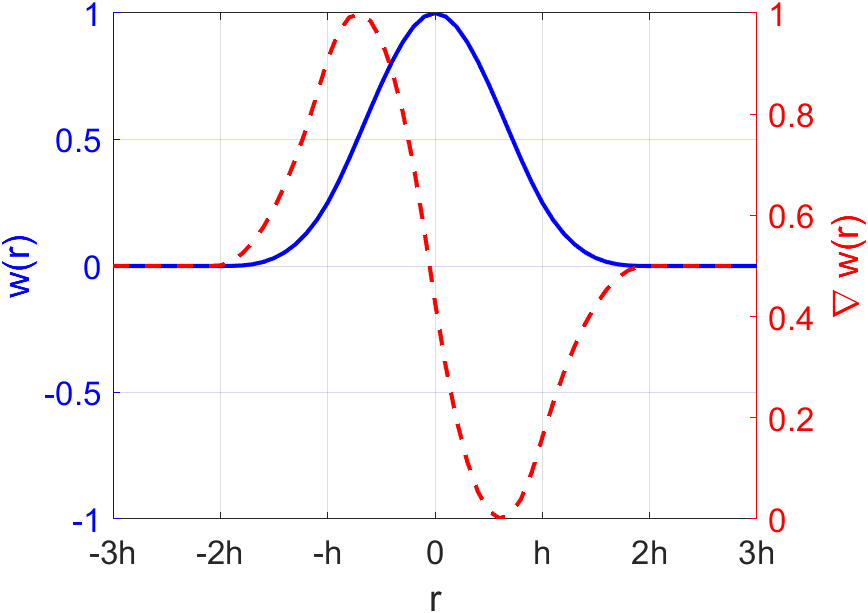
\includegraphics[height=35mm]{Figures/presentation_kernel}
\quad
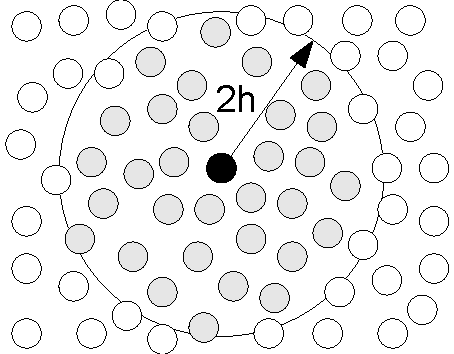
\includegraphics[height=35mm]{Figures/presentation_smoothing_length}}
%\vspace{5mm}
\item Pre-clustering to decrease time consumption from $O(n^2)$ to $O(m\cdot n)$ ($n$, $m<< $ total number of particles $n$)
\end{itemize}
\end{frame}

\subsection{Contact algorithm}
\begin{frame}
\frametitle{Contact algorithm}
\begin{itemize}
\item Penalty-based contact force ${\bm F}={\bm F}_n{\bm n}+f\mid{\bm F}_n\mid{\bm t}$ \\ ${\bm F}_n=k_{lin}p+k_{non}p^3$
\vspace{2mm}
\item Detecting particles within contact thickness $h_c$
\begin{itemize}
\item ${\bm F}$ acts on particle
\item $-{\bm F}$ acts on boundary element
\end{itemize}
\end{itemize}
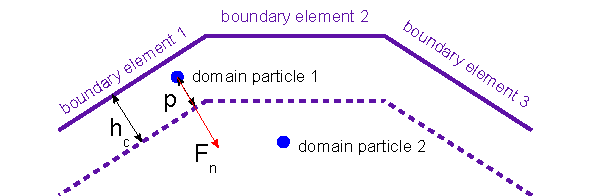
\includegraphics[height=35mm]{Figures/figure_contact}
\end{frame}

\section{Numerical simulation}
\begin{frame}
\frametitle{Numerical simulation}
\begin{itemize}
\item Kolsky impact bar impact compression setup (Casem et. al, 2014)
\begin{itemize}
\item Diameter and height 6.35 mm
\item Uniform particle spacing 0.254 mm
\item Only quarter of cylinder considered (symmetry)
\end{itemize}
\vspace{2mm}
\hspace{5mm}
\begin{minipage}[c]{4cm}\centering
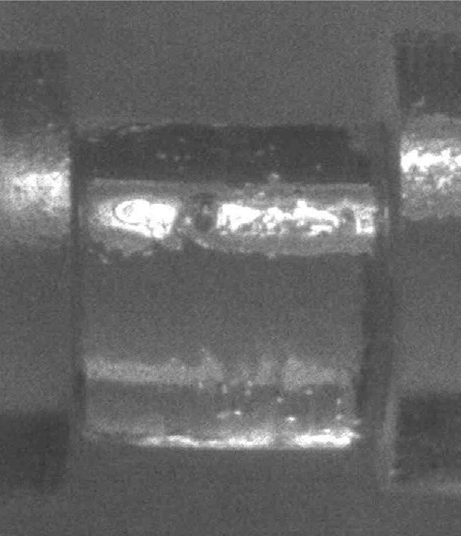
\includegraphics[height=35mm]{Figures/figure_experiment_0.png} \\
{\scriptsize\it Source: Casem et. al, 2014}
\end{minipage}
\hspace{2mm}
\begin{minipage}[c]{4cm}\centering
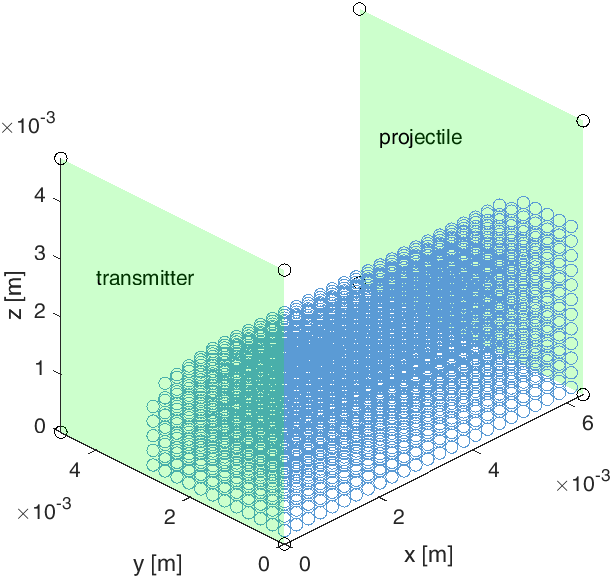
\includegraphics[height=40mm]{Figures/figure_setup.png}
\end{minipage}
\vspace{2mm}
\item Total number of 3025 particles
\end{itemize}
\end{frame}

\subsection{Constitutive parameters}
\begin{frame}
\frametitle{Constitutive parameters}
\begin{itemize}
\item Ballistic gelatine material data
\begin{center}
\begin{tabular}{c|c|c|c|c}
$\rho$ (kg/m$^\mathrm{3}$) & $E$ (Pa) & $\nu$ (-) & $K$ (Pa) & $G$ (Pa) \\
\hline
860 & 233300 & 0.49 & 3889000 & 78300
\end{tabular}
\end{center}
\vspace{5mm}
\item Constitutive parameters
\begin{center}
\begin{tabular}{c|c|c|c|c|c}
$\alpha$ (-) & $\beta$ (-) & $C_0$ (Pa) & $E_n$ (J/m$^\mathrm{3}$) & $s$ (-) & $\Gamma_0$ (-) \\
\hline
1.2 & 0 & 1520 & 0 & 1.87 & 0.18
\end{tabular}
\end{center}
\vspace{5mm}
\item Contact parameters
\begin{center}
\begin{tabular}{c|c|c|c}
$h_c$ (m) & $k_{lin}$ (N/m) & $k_{non}$ (N/m$^\mathrm{3}$) & $f$ (-) \\
\hline
1.143e$^\mathrm{-4}$ & 2.067e$^\mathrm{-2}$ & 0 & 0 \\
\end{tabular}
\end{center}
\end{itemize}
\end{frame}

%%%%%%%%%%%%%%%%%%%%%%%%%%%%%%%%%%%%%%%%%%%%%%%%%%%%%%
\section{Results}
\subsection{Comparison to experimental data}
\begin{frame}
\frametitle{Results}
\begin{itemize}
\item Constant velocity 6.35 m/s (boundary condition) corresponding to strain rate $\dot\epsilon = 1000 s^{-1}$
\item Transmitting force (contact force on boundary) to calculate sample stress $\sigma=\frac{F}{A}$ corresponding to sample strain $\epsilon=t\dot\epsilon$ \\
\vspace{2mm}
\hspace{5mm}
\begin{minipage}[c]{4cm}\centering
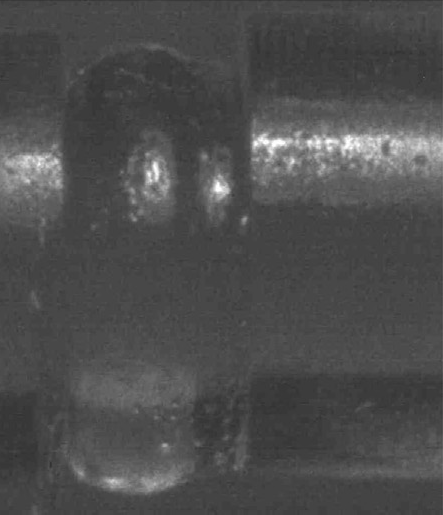
\includegraphics[height=35mm]{Figures/figure_experiment_T.png} \\
{\scriptsize\it Source: Casem et. al, 2014}
\end{minipage}
\hspace{2mm}
\begin{minipage}[c]{4cm}\centering
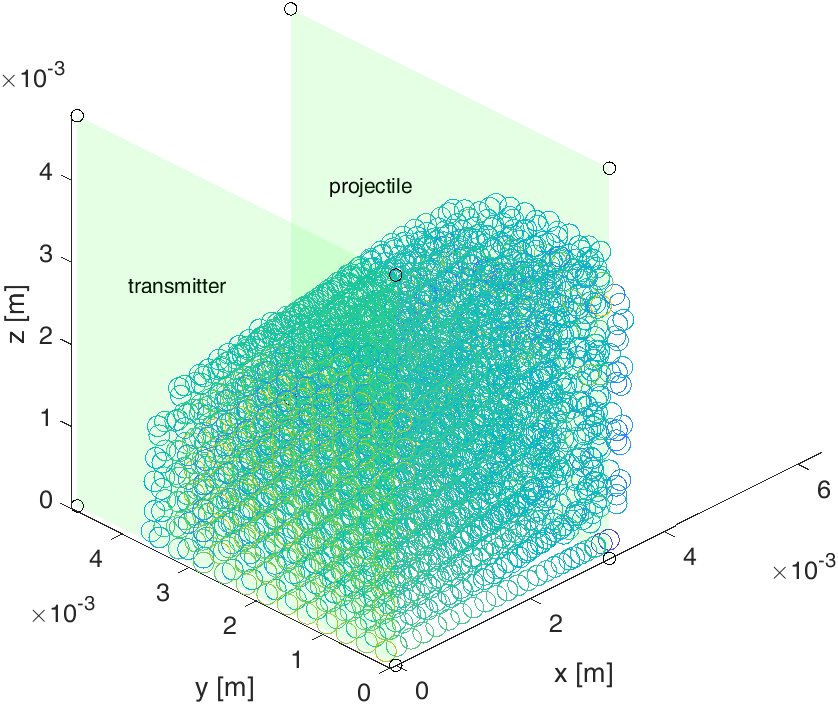
\includegraphics[height=40mm]{Figures/figure_compression.png}
\end{minipage}
\vspace{2mm}
\item Obvious non-uniform deformation in experiment
\end{itemize}
\end{frame}

%%%%%%%%%%%%%%%%%%%%%%%%%%%%%%%%%%%%%%%%%%%%%%%%%%%%%%
\begin{frame}
\frametitle{Results}
\begin{itemize}
\item Transmitting force
\end{itemize}
\centering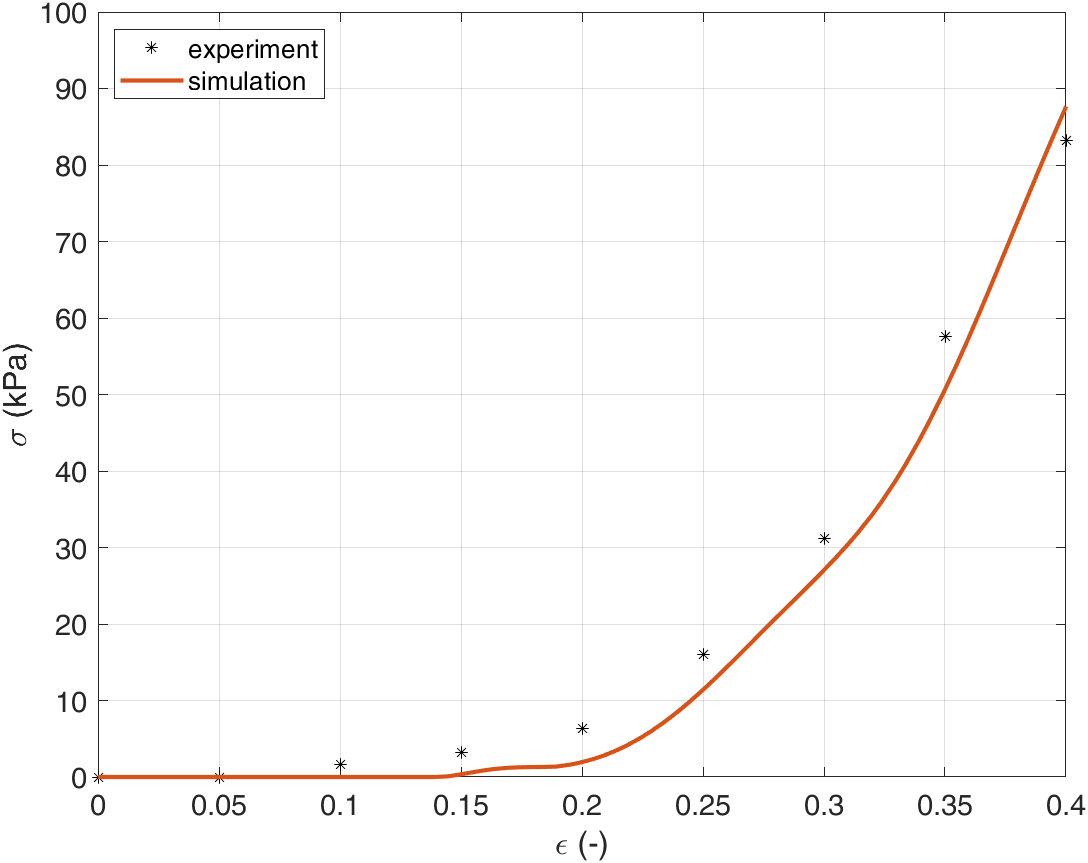
\includegraphics[width=8cm]{Figures/figure_comparison}
\end{frame}

%%%%%%%%%%%%%%%%%%%%%%%%%%%%%%%%%%%%%%%%%%%%%%%%%%%%%%
\section{Conclusion}
\subsection{Acknowledgements}
\begin{frame}
\frametitle{Conclusion}
\begin{itemize}
\item SPH implemented for ballistic gelatine numerical model
\item Generic material properties of ballistic gelatine
\item Numerical simulations verified the material model
\end{itemize}
\vskip5mm
{\small\color{myblue}This research was funded by the European Regional Development Fund-Project "Application of modern technologies in medicine and industry" (grant number CZ.02.1.01/0.0/0.0/17\_048/0007280).}
\end{frame}

\end{document}
